\section{Preliminaries and Policies Supported}
\begin{figure}
	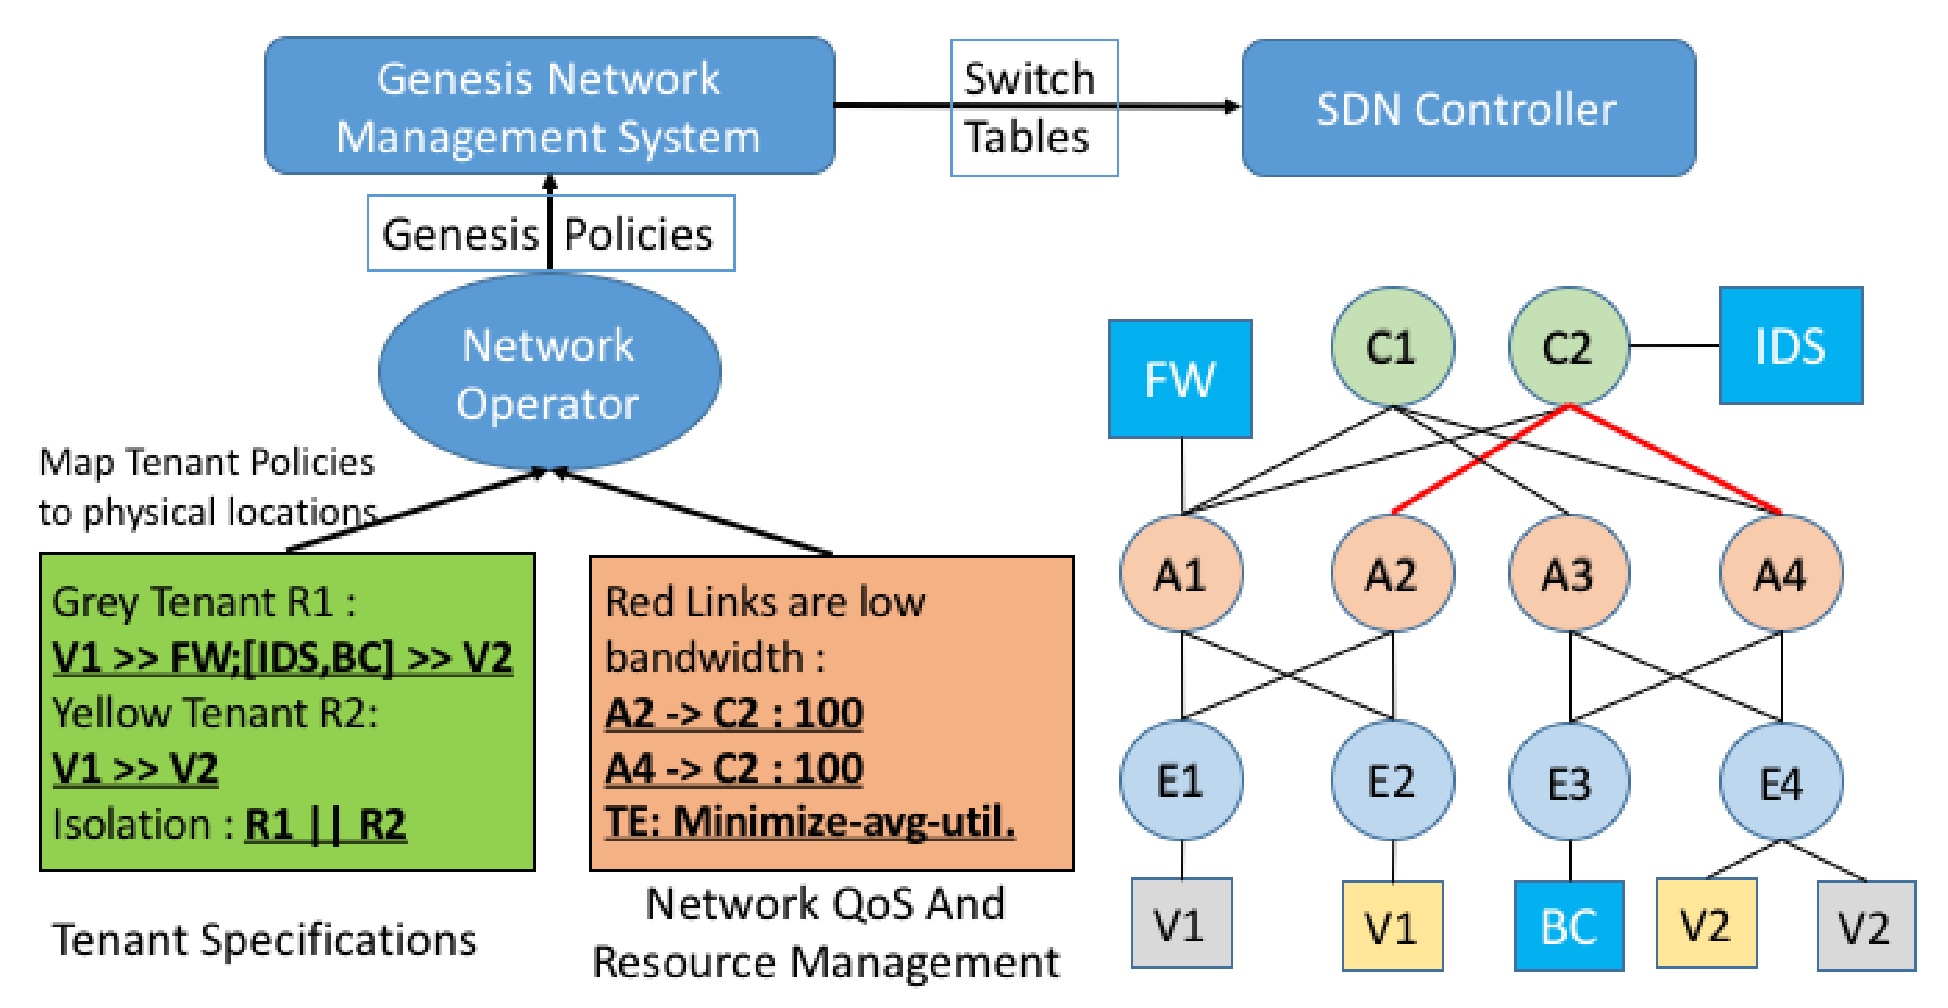
\includegraphics[width=\columnwidth,center]{figures/architecture.eps}
	\compactcaption{\Name in a multi-tenant datacenter setting of a network
		containing several VMs and middleboxes. The network operator translates
		the tenant specifications and network resource policies to \name 
		policies and \name synthesizes switch forwarding rules which are
		installed by the SDN controller.}
	\label{fig:architecture}
\end{figure}

\begin{table}[!t]
\begin{small}
	\begin{center}
		\begin{tabular}{m{7.8em}  m{15.9em} } 
			{\bf Policy} & {\bf Description} \\ 
			\hline
			Reachability & There is a path from router $src$ to router $dst$ for destination $\lambda$ \\ \hline
			Reachability with \newline Ordered Waypoints & The path  from $src$ to $dst$ for destination $\lambda$ 
			traverses some switch in the set $W_1$, \ldots, then some switch in the set $W_k$.\\ \hline
			Traffic Isolation & Paths of two reachability policies $R1$ and $R2$ do not share  links \\ \hline
			Traffic Engineering  & Minimize total/max link utilization \\
		\end{tabular}
	\end{center}
	\compactcaption{\genesis path-based policy support.} \label{tab:policysupport} 
\end{small}
\end{table}


%\section{Policy Support} \label{sec:policy}
%We design a language GPL (Genesis Policy Language) for network operators to express the desired end-to-end policies in a declarative manner which is interpreted by the Genesis synthesizer to find the forwarding rules for the network topology which enforce the input policies (\cref{fig:arch}). Genesis supports the following policies : 
%% Figure of GPL's syntax
%\begin{enumerate} 
%	\item \textbf{Reachability}: $predicate : src >> dst$ \\
%	This policy specifies the packets satisying $predicate$ have ingress router $src$ and egress router $dst$, and requires rules forwarding packets satisfying $predicate$ from $src$ to $dst$. There must be no forwarding loops in the network. 
%	\item \textbf{Waypoint}: $predicate : src >> W >> dst$ \\
%	The waypoint policy is a stronger reachability policy, and specifies that packet satisfying $predicate$ with ingress router $src$ and egress router $dst$ must pass through the set of waypoints $W$ in no particular order. The waypoint policy helps operators and tenants to specify the middleboxes the packets must traverse through without worrying about order, or having to use header tags to enforce a particular order \cite{flowtags}. 
%	\item \textbf{Traffic Isolation}:  $R1 \ || \ R2$ \\
%	The traffic isolation policy ensures that the . This policy can be used to provide fairness guarantees, since the paths of $R1$ and $R2$ don't share a link, the bandwidth used by $R1$ will not affect the bandwidth used by $R2$ and vice-versa. The condition of sharing a link in the same direction is due to the fact that links are full-duplex so, traffic flowing in one direction is not affected by the traffic flowing in the other direction.
%	\item \textbf{Security Isolation}: $R1 <> R2$ \\
%	The security isolation policy is stronger than the traffic isolation policy, and ensures that the path of the reachabiltiy/waypoint policies $R1$ and $R2$ do not share a link in both directions for increased security.
%	\item \textbf{}: $sw_1 \rightarrow sw_2 : capacity$ \\
%	The link capacity policy specifies that the capacity for link $sw_1 \rightarrow sw_2$ is $capacity$, and the weights of flows traversing the link in the direction of $sw_2$ do not exceed the capacity of the link.  
%	\item \textbf{Switch Table Size}: $sw : size$ \\
%	The router table size policy is used to specify the size of the forwarding table of the router $sw$ and ensures that the number of flows traversing through $sw$ does not exceed $size$ as each flow would require a forwarding rule at the switch.
%\end{enumerate}


We describe the type of policies desired in multi-tenant data centers
that \Name supports. We use \Cref{fig:architecture} as a running
example. In our setting, an ``operator'' manages a multi-tenant
datacenter, which could be either a public datacenter (E.g., Azure),
or a private datacenter. The operator specifies objectives that pertain
to how she wishes to manage her overall infrastructure.
%% For simplicity, we assume a multi-tenant cloud set up, where both
%% the tenants and the provider wish to realize policies over their
%% respective networks. However, these policies, and our framework,
%% are applicable to other settings, e.g., enterprise networks with
%% different departments imposing different sets of policies.
 A tenant is an entity (e.g., an enterprise or a department thereof)
 that has offloaded its IT infrastructure to the datcenter. Each
 tenant controls a number of host machines in the datacenter running
 some of its applications, and specifies policies that define whether
 paths can exist among it's hosts, and if so, what additional
 properties the paths must satisfy for security, performance or access
 control reasons. \Cref{fig:architecture} shows several tenants who
 differ in the nature of policies they wish to realize; we also show
 the operator's objectives.

 The policies and objectives supported by \Name are as described
 below. Notice that these reflect and, in some cases, extend policies
 and objectives that today's enterprises and datacenter operators
 realize in their networks~\cite{mpa-imc15}.

%\aditya{explain the figure here}.
%\kausik{Will do this now}

%\aditya{define flow, flow group, policy etc here}
% \aditya{need to start by saying we focus on multi-tenant clouds, although our system can apply elsewhere too}

% Operators of enterprise and multi-tenant clouds deal with policy
% requirements of different organisations and tenants, as well as
% require support to manage the network for providing QoS guarantees and
% network resource management internally, invisible to the
% tenants. Network operators need to be able to express complex policies
% in an intuitive declarative fashion, and the network management system
% must derive the individual switch forwarding behavior without
% involving the operator.


\begin{compactitemize}
\item \textbf{Tenant Policy: Reachability}. This enables network communication
  between specific pairs of a tenant's virtual instances (VMs),
  applications, or hosts.  In our example, one tenant has defined a
  reachability policy for its two VMs (R2): \texttt{V1 >> V2}, which
  is translated after VM placement (which is handled transparently by
  the operator) as $E2 >> E4$. A pair of VMs, applications or hosts
  that are allowed to communicate by means of a reachability policy
  defines a flow or a ``packet class''; we use these terms
  interchangeably. Any communication that is not defined by a
  reachability policy is implicitly blocked (i.e., all communication
  is ``default off'').
  
\item \textbf{Tenant Policy: Middlebox Traversals}. A tenant may wish that the flow
  between two of her end hosts, or from another tenant, must traverse
  specific middleboxes, which we also refer to as ``waypoints'' in
  this paper. Middleboxes are custom processing appliances often used
  for security, access control, or performance reasons (e.g.,
  firewalls, intrusion prevention systems, monitoring/accounting
  gateways, proxies, and load balancers). Specifically, for particular
  flows of interest, a tenant can provide a sequence of unordered sets
  of middleboxes
  %\loris{flow group is not defined, group of flows or set of flows?}
  to traverse~\cite{pga}. The flows must traverse these sets in order,
  while in a set, all middleboxes must be traversed and the order is
  irrelevant.\footnote{The unordered set abstraction leverages the
    fact that middleboxes without dependencies in their traffic
    processing behavior can be placed in any order relative to each
    other~\cite{pga}.} For example, one of the tenants defines a
  traversal policy (R1): $V1 >> FW; [IDS,BC] >> V2$ which specifies
  that traffic must first pass through the firewall (FW), and then
  through the Intrusion detection system (IDS) and the byte counter
  (BC) in any order.

  %% \aditya{refer here to an example in
  %%   the figure} In several cases \loris{how true is this?} the order
  %% in which these middle-boxes is traversed is not relevant and the
  %% policy language should therefore support unordered waypoints.

\item \textbf{Tenant Policy: Isolation}. Tenants may require various
  Quality-of-Service (QoS) or security guarantees that stipulate
  varying degrees of isolation for their traffic. In the extreme, a
  tenant could require that her flows are not affected in any manner
  by any other tenant by strictly isolating the path of the tenant's
  flows from others' flows. In \Cref{fig:architecture}, we have two
  tenants whose traffic will be isolated from one another, i.e., the
  network paths used by the tenants will not share any links in the
  topology.  A tenant could also specify isolation for a subset of her
  (performance-sensitive) flows from other flows of the same tenant or
  those belonging to other tenants; the rest of the tenant's flows may
  require no guarantees.

%%   There has been a rising emergence of 
%% multi-tenant clouds, which is more economical for tenants to use
%% rather than managing their own private datacenters. However,
%% the current Service Level Agreements (SLAs)
%% provided to tenants are centered around compute, storage, or
%% external traffic bandwidth. Lack of guarantees on the network
%% between tenant instances leads to unpredictability of performance
%% for distributed applications. Also, multi-tenant clouds are
%% susceptible to attacks on the network by malicious tenants who could
%% hog the internal network bandwidth, or conduct side-channel
%% attacks~\cite{heyyou-ccs}.
% Conventionally,
% this problem is mitigated by static rate-limiting, but it can lead
% to under-utilisation of resources.
%% Cloud provider can offer (paying) tenants various QoS guarantees
%% that enforce varying degrees of tenant isolation. In the extreme,
%% this could ensure that a tenant's performance is not affected by
%% any other tenant by strictly isolating the path of tenant's flows
%% from others' flows. \aditya{refer here to an example in
%% 	the figure} The tenant could also specify isolation for certain
%%  performance-sensitive flows, while the rest of the tenant-flows
%%   would be without guarantees with varying degrees of pricing. 
%%   Thus, support for isolation is an important feature in multi-tenant 
%%   networks. 
 
%TODO : MODIFY Synthesis of waypoints to support logical waypoints
%% Since, cloud tenants do not have a view of the actual physical
%% topology, the policy requirements for tenants are at a coarser level
%% of control. While support for the above policies can be used to satisfy tenant
%% SLAs, network operators can benefit from a fine-grained
%% control of network resources, integrated with support for tenant specifications 
%% for effective management of the network. \newline

%\loris{is there a reason why this is not in the itemize?} 
%\kausik{This is not a tenant policy, but an operator feature, so separate from itemize.}
\item \textbf{Operator Objective: Managing Capacity Constraints}. While support
  for the above policies can be used to satisfy tenant SLAs
  (service-level agreements), network operators often wish to
  carefully managing constrained resources. Common examples that \Name
  supports include enforcing strict constraints on aggregate number of
  flows traversing a switch (due to all tenants) so as to adhere to
  switch memory constraints, and ensuring that the total load on
  certain links is within predefined thresholds (we assume here that
  each flow has a predefined load). In our example in
  \Cref{fig:architecture}, A2-C2 and A4-C2 links are of low bandwidth,
  and the operator wants to ensure that total load on these links does
  not exceed 100.

\item \textbf{Operator Objective: Traffic Engineering}. As an alternative to
  managing strict (link) capacity constraints, operates may also want
  to balance load on their network infrastructure. This is often done
  by optimizing a network-wide objective such as total or maximum
  utilization of network links due to traffic induced by all tenants.
  
%For instance, to aid traffic engineering, the network
%operator may specify policies constraining the maximum number of
%tenant flows that can traverse a given link or sets of links in the
%network. She may also wish to ensure that traffic from some sensitive
%applications does not contend for bandwidth on constrained links with
%elastic traffic from batch applications. For example, in \Cref{fig:architecture},
%there are two low-bandwidth links in the datacenter, and the operator
%specifies policies to ensure that flows traversing $A2 \rightarrow C2$ 
%and $A2 \rightarrow C4$ do not exceed the link capacity of 100.
          %% capacity
          %% of certain links such that tenant flows using the link do
          %% not exceed the capacity of the link. Such policies can be
          %% useful to ensure the low bandwidth links are not used by
          %% more tenants such that their performance is affected and
          %% can be used to provide bandwidth guarantees to tenants.
  %% Likewise, to tackle hardware constraints, operators can specify
  %% switch constraints, e.g., restrict the number of flows traversing a
  %% particular switch or set of switches to adhere to switches'
  %% ruletable size limits.
  
 
 \item \textbf{Operator Objective: Handling failure gracefully}. Modern networks
   experience link and switch failures frequently~\cite{}.  When a
   failure occurs, we must reconfigure the forwarding rules such that
   the policies are satisfied. Naively recomputing forwarding rules
   incurs an unduly large overhead because old forwarding rules have
   to be torn down at all switches, and new rules installed. Switch
   rules deletions/insertions take a non-trivial amount of
   time~\cite{keqiang-sosr15}, potentially leading to disruptions. It
   is therefore desirable to have graceful approaches that either minimize the potential for disruption by minimizing the number of forwarding rules or switches
   modified in transitioning from an old data-plane,  or eliminate the possibility of disruption altogether by precomputing backup policy-compliant paths (at the cost of storing extra rules at switches).
   
   %% {\em minimal network repair} which
   %% aims to minimize the number of forwarding rules or switches
   %% modified in transitioning from an old data-plane to a new
   %% policy-compliant one to minimize disruption.  While repair is a
   %% reactive approach to failures, the transition {\em time} under
   %% failures can still be prohibitively high for some practical
   %% situations. Thus, as an alternative to minimal repair, it may be
   %% desirable to proactively configure switches with resilient
   %% policy-compliant backup paths; however this comes at the cost
   %% of additional switch rules.
\end{compactitemize}


\noindent Realizing these policies and objectives is challenging today.
%% legacy (non-SDN) networks
%% requires painstaking, often manual configuration of diverse network
%% devices. This is tedious---device configuration files can run into
%% 1000s of lines, and intricate dependencies may have to be configured
%% across devices~\cite{benson:complexity:nsdi2009,mpa-imc15}. This
%% process is also highly error prone~\cite{mpa-imc15}.
In particular, state-of-the-art SDN frameworks, e.g., Pyretic~\cite{}
and Frenetic~\cite{}, are insufficient to program networks to realize
them.  This is because the above policies/objectives are global and
cannot be enforced (at least not in an intuitive manner) by
programming individual behavior of switches.  While some existing
SDN-based network management systems~\cite{simple,merlin,oneswitch}
overcome these limitations by taking a network-wide view, they are
tailored to support specific policies such as middlebox placement or
link capacity constraints. As such they cannot enforce several of the
policies/objectives above.


\section{Data Plane Synthesis} \label{sec:synthesis} 

Our contribution is \name, a new general network management system
that supports the above policies and objectives, and can be extended
to support others. The architecture of \name is shown in
\Cref{fig:architecture}. \Name performs {\em synthesis} of switch
forwarding rules to enforce policies. The policies/objectives are
specified using Genesis Policy Language, or GPL, as shown in
\Cref{tab:policysupport}.

Unlike previous efforts in the network synthesis
space~\cite{netgen,merlin}, \Name is not tailored to specific
formalisms such as regular expressions; this aspect makes it {\em
  modular} and {\em easy to extend}.
%and allows to devise specific
%techniques for each type of policies. 
To draw an analogy with SMT solvers, \Name can be seen as a constraint
solver that allows the addition of different types of policies/objectives
(respectively, theories in SMT) and that allows the design of
optimizations based on the properties desired by network
  operators using \Name. 
  
  Our work is motivated by recent advances in program synthesis, i.e.,
  the task of discovering an executable program from user intent
  expressed in the form of some constraints. There are three key
  dimensions to a synthesis problem: the type of constraints that it
  accepts as expression of user intent, the space of programs over
  which it searches, and the search technique it employs.
  \Name\ leverages synthesis as follows: given a set of
  policies/objectives which describe tenant and operator intent, the
  search space is the space of all data planes (i.e., the set of
  forwarding rules) and the search technique involved is SAT/SMT
  solving.

\Name's approach has the following salient features:

(1) Enforcement of the different policies/objectives can be translated
to the following problem: Given a set of node pairs (derived from the
reachability policies) in the graph (topology), find paths in the
graph for each of the node pairs satisfying certain properties
(derived from the rest of the policies/objectives).  Thus, the
different policies/objectives can be enforced by a correct set of
forwarding rules at the switches.  No extra functionality is required
from the controller; its only role is to install the forwarding rules
on switches.

%Given these paths, the SDN
%controller adds the forwarding rules accordingly
%in the network, and no extra functionality is required from
%the controller. 
%Policies useful to operators are \emph{proactive} i.e., 
%for packets matching 

%they are not
%dependent on the actual packet flow and can be enforced by 
%correct switch tables, and do not require synthesis of controller programs.
%  and this enables enforcing policies by synthesis
% of switch-table rules, and using a skeleton SDN controller to deploy
% the forwarding rules to the switches. In contrast, in trying to
% synthesize reactive policies (like a firewall), the controller needs
% to store the state of flows it has received and have a control module
% following the specifications \aditya{huh? this doesn't make sense...},
% which is an interesting synthesis problem, but orthogonal to our
% approach.

(2) Correct enforcement is challenging due to different goals for each
of the policies/objectives --- ensuring isolation between paths may
lead to overshooting link utilizations and vice-versa --- and is a
common cause of incorrect configurations in networks.  Our approach
removes the need for a verification step in which the operator has to
``check'' whether the forwarding rules satisfy the desired
policies.  By using a formal reasoning technique, we are
able to consider the space of all data planes and find a solution
which is \emph{correct by construction}, eliminating room for operator
errors.


(3) Automatically enforcing policies is a task with
\emph{high theoretical complexity}.  For example, enforcing isolation
policies is as hard as solving graph-coloring, a well-known
NP-complete problem.  Many search techniques can be used to find the
forwarding rules when handling a particular class of policy, but when
multiple types of policies/objectives are combined, e.g., isolation, waypoints,
and traffic engineering, devising good search techniques becomes
challenging.  Thanks to the many engineering efforts, SMT solvers
abstract away most of this complexity and allow us to unify search
objectives for every policy into a generalized search technique.
%Thus, by reducing this problem to a SMT instance and
%leveraging fast off-the-shelf SMT solvers developed over years of
%research, \Name can provide support for diverse policies required by
%network operators. 
Crucially, \Name can be extended with ease to support new policies and
objectives without requiring changes to the underlying search
techniques.

In the next few sections, we describe the \Name synthesis
algorithm. In XXX we describe how \Name accommodates tenant policies.
We then describe how to accommodate operator objectives pertaining to
capacity constraints, traffic engineering and failure resiliency
(XXX).  Finally, we describe two novel \name techniques aimed at
speeding up \Name's synthesis: tactics (\secref{sec:tactic}) and
divide-and-conquer synthesis (\secref{sec:optimistic}).

%% \loris{I would like to convey that we are in some sense a Network solver module policy,
%% in the sense that we support theories (the policies) and now people can work on engineering
%% the solver for different classes of policies.
%% }
%% \kausik{To flow from this subsec to the next? Support for policies is 
%% 	inbuilt, but operators can engineer tactics to suit their needs. Is this what you want to convey?}
%% \loris{I found many words used to address the same concept:
%% enforce the policies, synthesize rules, etc...
%% try to be uniform or it's quite hard to understand what is being done.
%% } 
%% \kausik{I think "enforce policies" would be better? The title explains the rest.}


%\subsection{Performance Challenges} \label{sec:performance}
%
%\loris{I feel like this section is a repeat of the end of the intro.
%If you need a place to cut this is the one.
%I have a bit of the same feeling about 2.1 but that one at least motivates something.
%}
%
%One of the key challenges of \Name is the synthesis
%performance. 
%Due to the rich set of policies supported by \Name,
%finding a consistent set of switch forwarding rules 
%has, in the worst case, exponential time complexity in
%the number of policies.
%Moreover, since policies such as isolation affect
%the paths of many different flows, it is not possible to incrementally synthesize
%the forwarding rules corresponding to each flow. 
%Despite the recent advances in SMT solvers, to make
%the synthesis problem feasible in practice
%there is a need to improve the performance of the solver
%using techniques that are specific to policy enforcement in networks.
%We propose two such tecnhiques.
%
%First, we propose the idea of \emph{tactics} (\secref{sec:tactic}),
%which are search strategies that leverage the tiered network structure
%of datacenter topologies.
%%, to specify properties of the paths for the reachability
%%policies.  
%Tactics allow network operators to provide a high-level description on
%the set of paths allowed for reachability policies.  Tactics are
%expressed as simplified forms of regular expressions, which can be
%used to reduce the set of constraints provided to the solver.  In
%particular, we eliminate constraints that cannot be true for any
%of the paths accepted by the language of the regular expression. We
%find that this can result in 1.5x-400x speedup in various settings.
%
%Second, we propose a divide-and-conquer procedure that takes advantage of the fact that in 
%datacenter topologies, the large
%interconnect of links can lead to multiple solutions 
%to enforce the provided policies.  
%The divide-and-conquer
%synthesis approach (\secref{sec:optimistic}) leverages the structure of
%isolation policy graph among tenants to partition the input
%policies into components and synthesize these components separately and
%faster than the complete problem. This approach uses
% unsatisfiability cores provided by the solver
%to converge faster to the correct solution. 


